% Filename  : samplepaper.tex
% Purpose   : A sample exam paper to demonstrate how to use the 'ditpaper'
%             TeX class.
% Author    : Emmet Caulfield
% Revision  : $Id: samplepaper.tex 2 2006-02-19 20:34:45Z emmet $
% Repository: $HeadURL: http://svn.netrogen.lan/tex-ditpaper/trunk/samplepaper.tex $
%

% 'nosolution' (default) and 'solution' toggle the inclusion of solutions
% in the output. The tag solution, below, is replaced by 'sed' 
% in the Makefile to cause both the paper and the solutions to be produced.
\documentclass[solution]{ditpaper}
%\documentclass[solution]{ditpaper}


\usepackage{graphicx}
\usepackage{multirow}
\usepackage{rotating}


% These must be set or bizarre defaults will be used:
\facility{Kevin Street, Dublin 8}
\course{BSc. (Hons) in Computer Science}
\examcode{R228/419C}
\stage{Stage 4}
\session{Supplemental Examinations 2013}
\title{Artificial Intelligence II}
\examiners{Dr. John Kelleher\\
Dr. Deirdre. Lillis\\
Mr. D. Tracey}
\examdate{}
\examtime{Duration: 2 Hours}
\instructions{Question 1 is \textbf{compulsory}\par{} Answer Question 1 (40 marks) \textbf{and}\par{} any 2 Other Questions (30 marks each).}


\begin{document}


%aima chapters 18
% inductive bias, learning theory - supervised/unsupervised, overfitting, lazy/eager learner, classification v regression, false positive v false negatives, linear separability, consistency, evaluation

\question
\begin{enumerate}
	\item Explain what is meant by \textbf{inductive learning}.
	\marks{5}
	\begin{answer}
		Inductive Learning involves the process of learning by example where a system tries to induce a general rule from a set of observed instances
	\end{answer}
\item Describe the differences between \textbf{lazy learners} and \textbf{eager learners}, giving examples of each.
\marks{10}
		\begin{answer}
This is a discursive question so giving a precise answer is not appropriate. However, key points that the student should touch on include:\\
			Definitions:
			\begin{description}
				\item [Lazy learners] do not try to build a model from the training data, but simply use it at classification time
				\item [Eager learners] build a mode from the training data during training, and use only this model at classification time, ignoring the original data.
			\end{description}
			Key differences:
			\begin{itemize}
				\item Lazy methods may consider query instance when deciding how to generalise beyond the training data D; eager methods cannot since they have already chosen global approximation when seeing the query.
				\item \textbf{Efficiency} lazy learners require less training times but more time at prediction; eager learners require more training times by less time for prediction
				\item \textbf{Accuracy} lazy learners effectively uses a richer hypothesis space since it uses many local linear functions to form its implicit global approximation to the target function; eager learners must commit to a single hypothesis that covers the entire instance space.
				\item It is easier for lazy learners to handle \textbf{concept drift}
			\end{itemize}
			Examples:
			\begin{description}
				\item [Lazy learning example]: case based reasoning
				\item [Eager learning example]: Decision=tree, neural networks, support vector machines
			\end{description}
		\end{answer}
	\item  Inductive machine learning is often referred to as an \textbf{ill-posed problem}. What is meant by this?
	\marks{10}
	\begin{answer}
		Inductive machine learning algorithms essentially search through a hypothesis space to find a the best hypothesis that is consistent with the training data used. It is possible to find multiple hypotheses that are  consistent with a given training set (i.e. agrees with all training examples).  It is for this reason that inductive machine learning is referred to as an ill-posed problem as there is typically not enough information in the training data used to build a model to choose a single best hypothesis. Inductive machine learning algorithms must somehow choose one of the available hypotheses as the \emph{best}. An example like that shown in the figure below would be useful at this point
		\begin{center}
			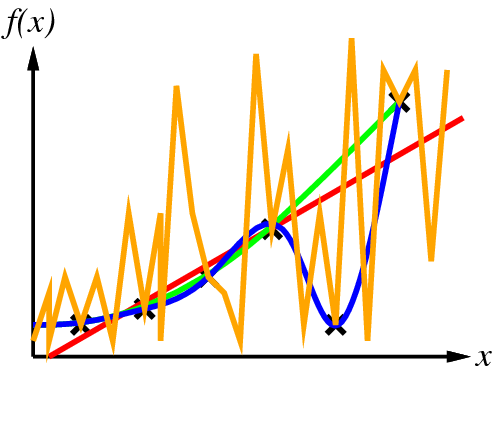
\includegraphics[width=5cm]{./images/curve-fitting5.png}
		\end{center}
	\end{answer}
\item Why is it difficult to select the correct inductive bias for a machine learning algorithm?
\marks{15}
\begin{answer}
This is a discursive question so giving a precise answer is not appropriate. However, key points that the student should touch on include:
		\begin{itemize}
			\item Choosing the correct inductive bias for a particular inductive learning problem is difficult because it involves getting the balance right in the \textbf{tradeoff} between the expressiveness of a hypothesis space and the complexity of finding a simple, consistent hypothesis within that space. In other words, there is a tradeoff between complex hypotheses that fit the training data well and simpler hypotheses that may \textbf{generalise} better (How well a model trained on a training set predicts the right output for new instances is called \textbf{generalization}).
			\item If the hypothesis class \H~is less complex than the true function we are trying to model, we have \textbf{underfitting}. In other words the inductive bias is to restrictive on the search and the learning algorithm is not able to generate hypotheses that are complex enough. In the case of underfitting, as we increase the complexity allowed by the inductive bias, (i.e., increase the complexity of \H) the training error decreases. 
			\item If our model selection has chosen a \H~that is too complex, the data is not enough to constrain it and we may end up with a bad hypothesis. Whenever there is a large set of possible hypotheses, one has to be careful not to use the resulting freedom to find meaningless ''regularity'' in the data. This problem is called \textbf{overfitting}. Overfitting becomes more likely as the hypothesis space and the number of input attributes grows, and less likely as we increase the number of training examples.
		\end{itemize}
\end{answer}



\end{enumerate}


\newpage

%Q2
% knn and CBR 
% information theory, entropy, Decision Trees, Inductive logic programming
		
\begin{table}[!tb]
\caption{A dataset showing the behaviour of two individuals in an online shop. A 1 indicates that the person bought the item a 0 indicates that they did not.}
\label{table:binaryDataset}
\centering
\begin{tabular}{ | c | c | c | c | c | c |}
\hline
Person ID & Item 107 & Item 498 & Item 7256 & Item 28063 & Item 75328\\
\hline
A  &  1 & 1 & 1 & 0 & 0\\
B  &  1 & 0 & 0 & 1 & 1\\
\hline \hline 
\end{tabular}
\label{tab:binarydata}
\end{table}

\begin{table}[!tb]
\caption{A query instance from the same domain as the examples listed in Table \ref{tab:binarydata}. A 1 indicates that the person bought the item a 0 indicates that they did not.}
\label{table:binaryDataset}
\centering
\begin{tabular}{ | c | c | c | c | c | c |}
\hline
Person ID & Item 107 & Item 498 & Item 7256 & Item 28063 & Item 75328\\
\hline
Q  &  1 & 0 & 1 & 0 & 0\\
\hline \hline 
\end{tabular}
\label{tab:binaryquery}
\end{table}

			
\question 
\begin{enumerate}
	\item You have been given the job of building a recommender system for an large online shop that has a stock of over 100,000 items. In this domain the behaviour of individuals is captured in terms of what items they have bought or not bought. Table \ref{tab:binarydata} lists the behaviour of two individuals in this domain for a subset of the items that at least one of the individuals has bought. Table \ref{tab:binaryquery} lists the behaviour of a customer that you want to generate recommendations for. Table \ref{tab:similaritymetrics} lists 3 different models of similarity that work on binary data, similar to the data in this domain (\textbf{Russell-Rao}, \textbf{Sokal-Michener}, and \textbf{Jaccard}).
	\begin{table}[h]
	\begin{center}
	\begin{tabular}{rl}
	Russell-Rao(X,Y) & $= \frac{CP(X,Y)}{P}$\\
	Sokal-Michener(X,Y) & $=\frac{CP(X,Y)+CA(X,Y)}{P}$\\
	Jaccard(X,Y) & $=\frac{CP(X,Y)}{CP(X,Y)+PA(X,Y)+AP(X,Y)}$\\
	\end{tabular}
	\end{center}
	\caption{Similarity Metrics for Binary Data.}
	\label{tab:similaritymetrics}
	\end{table}

	\begin{enumerate}
			\item Given that there are over 100,000 items available in the store which of these models of similarity (\textbf{Russell-Rao}, \textbf{Sokal-Michener}, or \textbf{Jaccard}) is most appropriate for this domain. Give an explanation for your choice.
	\marks{5}
	\begin{answer}
In a domain where there are 100,000's of items co-absenses aren't that meaningful. For example, you may be in a domain where there are so many items most people haven't seen, listened to, bought or visited the vast majority of them and as a result the majority of features will be co-absenses. The technical term to describe dataset where most of the features have zero values is \textbf{sparse data}. In these situations you should use a metric that ignore co-absenses and if your features are binary then you should use the \textbf{Jaccard similarity} index. 
	\end{answer}
			\item Assuming that the recommender system uses the similarity metric you selected in Part (i) and that the system will recommend to person Q the items that the person most similar to person Q has already bought but that person Q has not bought, \textbf{which item or items will the system recommend to person Q?} Support you answer by showing your calculations and explaining your analysis of the results.
	\marks{10}
	\begin{answer}
		Using a similarity metric the higher the value returned by the metric the more similar the two items are.\\
		Assuming the student chose the \textbf{Jaccard} similarity metric then Person A is more similar to Q than Person B: $Jaccard(Q,A) = \frac{2}{2+1}= 0.6667$, $Jaccard(Q,B) = \frac{1}{4}= 0.25$. As a result the system will recommend item \textbf{498}.\\
		If the student selected one of the other similarity metrics for part (a), the supporting calculations should be:
\begin{itemize}
	\item Russell-Rao(Q,A)$=\frac{2}{5}= 0.4$
	\item Russell-Rao(Q,B)$=\frac{1}{5}= 0.2$
	\item Sokal-Michener(Q,A)$=\frac{4}{5}= 0.8$
	\item Sokal-Michener(Q,B)$=\frac{2}{5}= 0.4$	
\end{itemize}
		As is evident from these calculations regardless of which similarity metric is used Person A is more similar to Q than Person B. So the system will recommend item \textbf{498} regardless of which similarity metric is used.
	\end{answer}

     \end{enumerate}

		% Information theory and Decision Trees
		\item Table \ref{tab:id3data}, on the next page lists a data set with of 6 examples described in terms of 3 binary descriptive features (\textbf{A}, \textbf{B}, and \textbf{C}) and a target label (\textbf{Target}). You are asked to create a decision tree model using this data. \textbf{Which of the descriptive features will the ID3 decision tree induction algorithm choose as the feature for the root node of the decision tree?} Support you anwer with appropriate calculations and dicussions of your results. Note that Table \ref{tab:info-eqs}, also on the next page, lists some equations that you may find useful for this question.		
		\marks{15}
		\begin{answer}
		The ID3 decision tree induction algorithm selects the decriptive feature with the highest information gain as the feature for the root node of the decision tree.  The first step in calculating information gain is to calculate the entropy for the entire dataset:
	\begin{eqnarray*}
H\left(DS\right) &=& - \sum_{v \in \{C1,C2\}} p_v ~ log_2 p_v\\
		&=& -\left(\frac{3}{6}~ log_2 \frac{3}{6}\right) + -\left(\frac{3}{6} ~log_2 \frac{3}{6}\right)\\
		&=& 1.00~bits
	\end{eqnarray*}
	The table below shows the calculation of the infromation gain for each of the descriptive features in the dataset:
		\begin{scriptsize}
\begin{tabular}{ccccccc}
Split & Feature &              &  & Entropy of &  & Info.\\
By & Value & Partition  & Examples & Partition & Remainder & Gain\\
\hline
\multirow{2}{*}{A} & 1 & $DS_1$  & 1,2,3 & 0.9183 & \multirow{2}{*}{0.9183} & \multirow{2}{*}{0.0817}\\
 & 0 & $DS_2$ & 4,5,6 & 0.9183 &  & \\
\hline
\multirow{2}{*}{B} & 1 & $DS_3$ & 2,4,5,6 & 0.8113 & \multirow{2}{*}{0.5409} & \multirow{2}{*}{0.4591}\\
& 0 & $DS_4$ & 1,3 & 0 &  & \\
\hline
\multirow{2}{*}{C} & 1 & $DS_5$ & 1,2,3,4,6 & 0.9709 & \multirow{2}{*}{0.8091} & \multirow{2}{*}{0.1909}\\
& 0 & $DS_6$ & 5 & 0 &  & \\
\hline
\end{tabular}
	\end{scriptsize}
	From this table we can see the feature \textbf{B} has the highest information gain and consequently the ID3 algorithm will chose this feature as the feature tested at the root node of the tree.
		\end{answer}

\begin{table}[htb]
\centerline{
\begin{tabular}{|c|c|c|c|c|}
\hline
\textbf{ID}	 & \textbf{A}	& \textbf{B} & \textbf{C} & \textbf{Target}\\
\hline
1 & 1 & 0 & 1 & C1\\
2 & 1 & 1 & 1 & C2\\
3 & 1 & 0 & 1 & C1\\
4 & 0 & 1 & 1 & C2\\
5 & 0 & 1 & 0 & C1\\
6 & 0 & 1 & 1 & C2\\
\hline
\hline
\end{tabular}
}
\caption{Dataset for the ID3 Algorithm Question}
\label{tab:id3data}
\end{table}

	\begin{table}[htb]
	\begin{center}
	\begin{tabular}{rl}
	Entropy(DS) & $= -\sum_{i=1}^k p_i \times log_2(p_i)$\\
	Remainder(F) & $=\sum_{v \in Domain(F)} \frac{|DS_v|}{|DS|} Entropy(DS_v)$\\
	InformationGain(F,DS) & $=Entropy(DS)-Remainder(F)$\\
	\end{tabular}
	\end{center}
	\caption{Equations from information theory.}
	\label{tab:info-eqs}
	\end{table}


	\end{enumerate}

\clearpage
\newpage
	
%Q3 30 marks
% basic probability 5
% bayesian networks 10
% bayesian learning  15

\begin{table}[!htb]
    \caption{Spam and Ham Dataset}
    \begin{minipage}{.5\linewidth}
      \centering
\begin{tabular}{l}
\textbf{Spam}\\
\hline
\textit{Offer is Free}\\
\textit{Free Learning Link}\\
\textit{Click Free Link}\\
\hline
\end{tabular}
    \end{minipage}%
    \begin{minipage}{.5\linewidth}
      \centering
\begin{tabular}{l}
\textbf{Ham}\\
\hline
\textit{Great Learning Fun}\\
\textit{Great Machine Learning}\\
\textit{Free Learning Event}\\
\textit{Learning is Fun}\\
\textit{Learning Costs Money}\\
\hline
\end{tabular}
    \end{minipage} 
    \label{tab:spamhamdata}
\end{table}

\begin{table}[h]
\caption{Query Title}
\centering
\begin{tabular}{l}
\hline
\textit{Fun is Free}\\
\hline
\end{tabular}
\label{tab:spamhamquery}
\end{table}


\question Table \ref{tab:spamhamdata} lists a dataset of email subjects. Table \ref{tab:spamhamquery} lists the title of a query instance that we would like to classify as being either a spam or ham email based on its title. 
	\begin{enumerate}
		\item Using \textbf{Laplacian smoothing}, where 
		\begin{eqnarray*}
		p(x=v) &=& \frac{count(x=v)+k}{count(x) +( k \times |Domain(x)|)}
		\end{eqnarray*}
		with \textbf{k=1} and a \textbf{vocabulary size of 12} calculate the following probabilities:
			\begin{enumerate}
				\item $P(Spam)=?$
				\marks{2}
					\begin{answer}
						$P(Spam) = \frac{3+1}{8 + (1 \times 2)} = \frac{4}{10} = 0.4$
					\end{answer}
				\item $P(Ham)=?$
				\marks{2}
					\begin{answer}
						$P(Ham) = \frac{5+1}{8 + (1 \times 2)} = \frac{6}{10} = 0.6$
					\end{answer}
				\item $P('Fun'|Spam)=?$
				\marks{2}
					\begin{answer}
						$P('Fun'|Spam) = \frac{0+1}{9 + (1 \times 12)} = \frac{1}{21} = 0.0476$
					\end{answer}
				\item $P('Fun'|Ham)=?$
				\marks{2}
					\begin{answer}
						$P('Fun'|Ham) = \frac{2+1}{15 + (1 \times 12)} = \frac{3}{27} = 0.1111$
					\end{answer}
				\item $P('is'|Spam)=?$
				\marks{2}
					\begin{answer}
						$P('is'|Spam) = \frac{1+1}{9 + (1 \times 12)} = \frac{2}{21} = 0.0952$
					\end{answer}
				\item $P('is'|Ham)=?$
				\marks{2}
					\begin{answer}
						$P('is'|Ham) = \frac{1+1}{15 + (1 \times 12)} = \frac{2}{27} = 0.0741$
					\end{answer}
				\item $P('Free'|Spam)=?$
				\marks{2}
					\begin{answer}
						$P('Free'|Spam) = \frac{3+1}{9 + (1 \times 12)} = \frac{4}{21} = 0.1905$
					\end{answer}
				\item $P('Free'|Ham)=?$
				\marks{2}
					\begin{answer}
						$P('Free'|Ham) = \frac{1+1}{15 + (1 \times 12)} = \frac{2}{27} = 0.0741$
					\end{answer}
			\end{enumerate}
		\item Calculate the probability of the query title in Table \ref{tab:spamhamquery} belonging to the Spam class under the \textbf{Naive Bayes assumption} and using the \textbf{smoothed probabilities} you calculated in Part (a):		
%Using the smoothed probabilities you calculated in Part 1 of calculate the probability under the \textbf{Naive Bayes assumption} of the query title in Table \ref{tab:songmoviequery} belonging to the Movie class:
			\begin{center}
				$P(Spam|'Fun~is~Free')=?$
			\end{center}
			\marks{8}
			\begin{answer}
				$P(Spam|'Fun is Free')$ 
				\begin{scriptsize}
				\begin{eqnarray*}
					&=& \frac{P('Fun'|Spam)P('is'|Spam)P('Free'|Spam)P(Spam)}{(P('Fun'|Spam)P('is'|Spam)P('Free'|Spam)P(Spam))+(P('Fun'|Ham)P('is'|Ham)P('Free'|Ham)P(Ham))}\\
					&=& \frac{0.0476 \times 0.0952 \times 0.1905 \times 0.4}{(0.0476 \times 0.0952 \times 0.1905 \times 0.4) + (0.1111 \times 0.0741 \times  0.0741 \times 0.6)}\\
					&=& 0.48543863
				\end{eqnarray*}
				\end{scriptsize}
			\end{answer}
		\item Calculate the probability of the query title in Table \ref{tab:spamhamquery} belonging to the Spam class under the \textbf{Naive Bayes assumption} and using \textbf{maximum likelihood} probabilities (i.e. the probabilities we would get if we did not use Laplacian smoothing):	
%Using \textbf{maximum likelihood} probabilities (i.e. do not use Laplacian smoothing in calculating the probabilities) calculate the probability under the \textbf{Naive Bayes assumption} of the query title in Table \ref{tab:songmoviequery} belonging to the Movie class:	
					\begin{center}
				$P(Spam|'Fun~is~Free')=?$
			\end{center}
			\marks{6}
			\begin{answer}
				Because the word 'Fun' does not appear in any of the Spam titles the maximum likelihood (i.e., unsmoothed) probability of $P('Fun'|Spam)=0$. As a result the maximum likelihood probability of $P(Spam|'Fun~is~Free')=0$. Showing the complete calculation: \\
				\\
				P(Spam|'Fun~is~Free')
				\begin{scriptsize}
				\begin{eqnarray*}
					&=& \frac{P('Fun'|Spam)P('is'|Spam)P('Free'|Spam)P(Spam)}{(P('Fun'|Spam)P('is'|Spam)P('Free'|Spam)P(Spam))+(P('Fun'|Ham)P('is'|Ham)P('Free'|Ham)P(Ham))}\\
					&=& \frac{\frac{0}{9} \times \frac{1}{9} \times \frac{3}{9} \times \frac{3}{8}}{(\frac{0}{9} \times \frac{1}{9} \times \frac{3}{9} \times \frac{3}{8})+(\frac{2}{15} \times \frac{1}{15} \times \frac{1}{15} \times \frac{5}{8})}\\
					&=& 0.0
				\end{eqnarray*}
				\end{scriptsize}
			\end{answer}
	\end{enumerate}
%
\newpage

%Q4
%Linear Regression Neural Nets, SVMs, Ensemble Learning
%Q4
%Linear Regression Neural Nets, SVMs, Ensemble Learning


\question 
	\begin{enumerate}
		\item The following model is commonly used for continuous prediction tasks:

\begin{center}
$y(x)=w_0 + w_1x_1 + \dots + w_Dx_D$
\end{center}

\begin{enumerate}
\item Provide the name for this model and explain all its terms.
	\marks{3}


		\begin{answer}
		Students should explain that this is a simple linear regression model which can be effectively used to make predictions. $x$ is a vector of feature values for a query instance and $w$ is a vector of feature weights. An diagram of a simple one dimensional linear function would help.
		\end{answer}
		
\item Briefly describe a technique for finding optimal values for the terms\\ $w_0, w_1, \dots , w_D$ in the model based on a historical training set.
	\marks{3}

		\begin{answer}
		
		Students should explain that given a training set the performance of a particular linear regression model can be measured using an appropriate evaluations function, e.g. the \emph{sum of squares error} as follows:
		
		\begin{center}
		$E(w)=\frac{1}{2}\sum_{n=1}^{N}(y(x_n)-t_n)^2$
		\end{center}
				
		where $t_n$ is the \emph{true} answer for training instance $x_n$ and $y(x_n)$ is the prediction made by the model for instance $x_n$. Optimal values for $w$ are found by minimising E(w).
		\end{answer}
\end{enumerate}
		
		%Neural Nets	
		\item Figure \ref{fig:nn}, on the next pages, shows a backprogation network that is currently processing the training vector $[1.0, 0.9, 0.9]$ which has an  associated target vector $[0.1, 0.9, 0.1]$. Given that the output from unit B is $0.6$ and from C is $0.8$, and assuming that the activation function used at all nodes in the network is the logistic function, carry out the calculations listed below. Note that Table \ref{tab:nn-eqs}, also on the next page, lists some equations that you may find useful when doing this question. 
\begin{enumerate}
	\item Calculate the actual output vector (to 3 decimal places).
	\marks{10}
		\begin{answer}
		%Output of unit $x = a_x(in_x) = \frac{1}{1 + \exp^{-\sum_j W_{jx} a_j(in_j)}}\\
		%First output unit input $i$\\
		\begin{eqnarray*}
		a_i(in_i) &=&\frac{1}{1 + \exp^{- ((W_{BD} \times a_B(in_B) + (W_{CD} \times a_C(in_C) ))}}\\
		&=&\frac{1}{1 + \exp^{- ((-0.3 \times 0.6) + (0.9 \times 0.8}))}\\
		&=&\frac{1}{1 + \exp^{- 0.54}}\\
		&=&0.632
		\end{eqnarray*}
		%Second output unit input $j$\\
		\begin{eqnarray*}
		a_j(in_j) &=&\frac{1}{1 + \exp^{- ((W_{BE} \times a_B(in_B) + (W_{CE} \times a_C(in_C) ))}}\\
		& = &\frac{1}{1 + \exp^{- ((-0.6 \times 0.6) + (0.1 \times 0.8}))}\\
		& = &\frac{1}{1 + \exp^{- (-0.44)}}\\
		& = &0.392
		\end{eqnarray*}
		%Third output unit input $k$\\
		\begin{eqnarray*}
		a_k(in_k) &=&\frac{1}{1 + \exp^{- ((W_{BF} \times a_B(in_B) + (W_{CF} \times a_C(in_C) ))}}\\
		& = &\frac{1}{1 + \exp^{- ((0.4 \times 0.6) + (1.2 \times 0.8}))}\\
		& = &\frac{1}{1 + \exp^{- 1.2}}\\
		& = &0.769
		\end{eqnarray*}
		\end{answer}
	\item Calculate the \textbf{$\Delta$} error for each output unit (to 3 decimal places).
	\marks{6}
		\begin{answer}
		\begin{eqnarray*}
		\Delta_D& = &(target_D - a_D(in_D)) \times a_D(in_D) \times (1-a_D(in_D))\\
		& = &(0.1-0.632) \times 0.632 \times (1-0.632)\\
		& = &-0.124
		\end{eqnarray*}
%		Second output unit $j$\\
		\begin{eqnarray*}
		\Delta_E& = &(target_E - a_E(in_E)) \times a_E(in_E) \times (1-a_E(in_E))\\
		& = &(0.9-0.392) \times 0.392 \times (1-0.392)\\
		& = &0.121
		\end{eqnarray*}
%		Third output unit $k$\\
		\begin{eqnarray*}
		\Delta_F& = &(target_F - a_F(in_F)) \times a_F(in_F) \times (1-a_F(in_F))\\
		& = &(0.1-0.769) \times 0.769 \times (1-0.769)\\
		& = &-0.119
		\end{eqnarray*}
		\end{answer}
	\item Calculate the \textbf{$\Delta$} error for each hidden unit B and C. (to 3 decimal places)
		\marks{8}
		\begin{answer}
%Again we are using backprop to train a multi-layer network so we use the Delta error rules. In this case the Delta error rule for hidden units. Each hidden node $j$ is responsible for some fraction of the error $\Delta_i$ of each of the output units $i$ to which it connects. Thus the $\Delta_i$ values are divided according to the strengths of the connection between the hidden node and the output nodes and are propagated back to the hidden nodes. Where a hidden node feeds-forward into more than 1 output node the errors propagated back to it are summed. So the error for a hidden unit $j$ feeding into $n$ units= $\Delta_j = a_j(in_j) \times (1-a_j(in_j)) \times \left( \sum_{i=1}^{n}W_{ji} \times \Delta_i \right)$\\
\begin{eqnarray*}
\Delta_B &=& a_B(in_B) \times (1-a_B(in_B)) \times \left( \sum_{x \in \{D,E,F\}}^{n}W_{Bx} \times \Delta_x \right)\\
&=& a_B(in_B) \times (1-a_B(in_B)) \times \left(((W_{BD} \times \Delta_D)+(W_{BE} \times \Delta_E)+(W_{BF} \times \Delta_F))\right)\\
&=& 0.6 \times (1-0.6) \times \left(((-0.3 \times -0.124)+(-0.6 \times 0.121)+(0.4 \times -0.119))\right)\\
&\approx& -0.020\\
\end{eqnarray*}

\begin{eqnarray*}
\Delta_C &=& a_C(in_C) \times (1-a_C(in_C)) \times \left( \sum_{x \in \{D,E,F\}}^{n}W_{Cx} \times \Delta_x \right)\\
&=& a_C(in_C) \times (1-a_C(in_C)) \times \left(((W_{CD} \times \Delta_D)+(W_{CE} \times \Delta_E)+(W_{CF} \times \Delta_F))\right)\\
&=& 0.8 \times (1-0.8) \times \left(((0.9 \times -0.124)+(-0.1 \times 0.121)+(1.2 \times -0.119))\right)\\
&\approx& -0.043\\
\end{eqnarray*}

		\end{answer}
%	\item Calculate the new weight $W_{BD}$ for the connection from unit B to the output unit D after the training example has been processed. Use a learning rate of $\eta = 0.25$.
%		\marks{4}
%		\begin{answer}
%		\begin{eqnarray*}			
%		W_{B,D} &=& W_{B,D} + (\eta \times a_B(in_B) \times \Delta_D)\\
%				&=& -0.3 + (0.25 \times 0.6 \times -0.124)\\
%		           &=& -0.319
%		\end{eqnarray*}
%	\end{answer}
\end{enumerate}

\end{enumerate}

\clearpage
\newpage

\begin{figure}[htbp]
\begin{center}
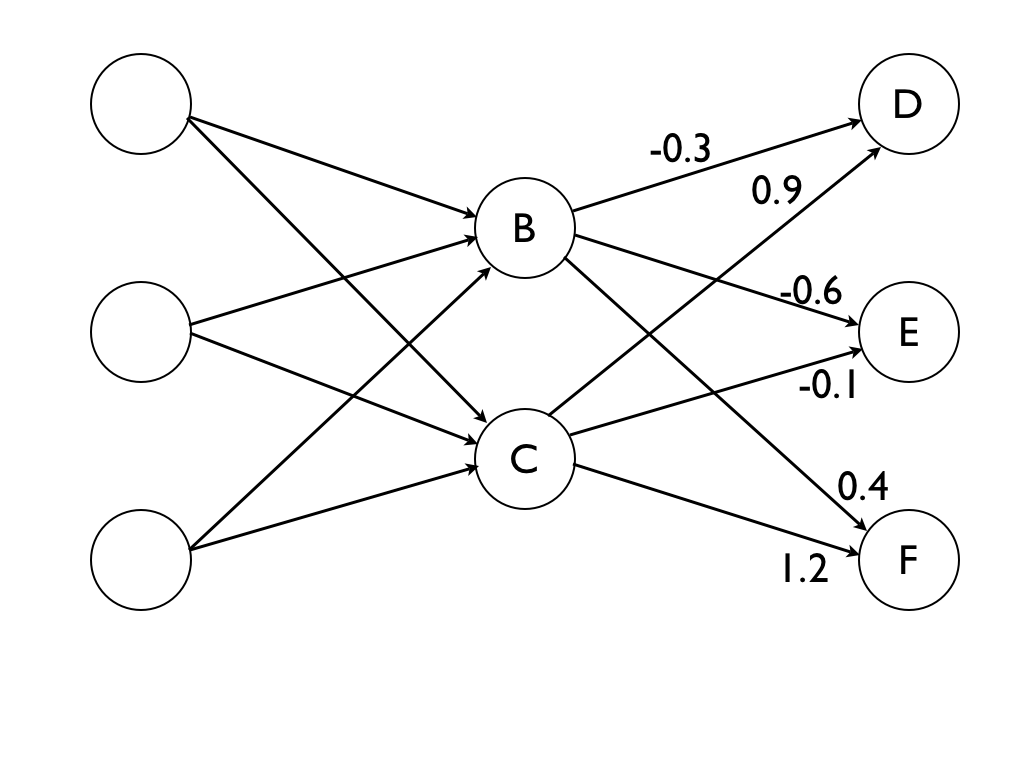
\includegraphics[width=3.5in]{./images/backpropnetwork1.png}
\caption{Example Neural Net}
\label{fig:nn}
\end{center}
\end{figure}

	\begin{table}[htb]
	\begin{center}
	\begin{tabular}{ll}
	Weighted sum of inputs for unit $i$ with $j$ inputs:  & $in_i = \sum_j W_{ji} a_j(in_j)$\\
	Activation Function (Logistic) for unit $i$: & $a_i(in_i) = \frac{1}{1 + \exp^{-in_i}}$ \\
	Perceptron weight update rule for link  $j\rightarrow i$ & $w_{ji}=w_{ji} + \eta \left( t_i - a_i(in_i) \right) \times a_j(in_j)$\\
      Hebbian Weight Update Rule for link  $j\rightarrow i$ & $w_{ji} = \eta \times a_j(in_j) \times a_i(in_i)$\\
	Partial Derivative for Logistic Activation Function & $\frac{\delta a_i(in_i)}{\delta in_i}=a_i(in_i) \times (1-a_i(in_i))$\\
	Error for an output unit $i$ & $error_i =  target_i - a_i(in_i)$\\
	Delta Error for an output unit $i$ & $\Delta_i =  error_i \times a_i(in_i) \times (1-a_i(in_i))$\\
	Delta Error for a hidden unit $j$ feeding into $n$ units & $\Delta_j = \left( \sum_{i=1}^{n}W_{ji} \times \Delta_i \right) \times a_j(in_j) \times \left(1-a_j(in_j)\right)$\\
      Delta Weight Update Rule for link $x \rightarrow k$ & $W_{x,k} = W_{x,k} + (\eta \times a_x(in_x) \times \Delta_k)$\\
	\end{tabular}
	\end{center}
	\caption{Equations used in Perceptron and Neural Network training.}
	\label{tab:nn-eqs}
	\end{table}
\end{document}
